\documentclass[mathserif, aspectratio=169]{beamer}
%
%%%%%%%%%%%%%%%%%%%%%%%%%%%%%%%%%%%%%%%%%%%%%%%%%%%%%%%%%%%%%%%%%%%%%%%%
% need to split the includes to make spell checking work.
\usepackage{arev, arevmath}
\usepackage[scaled]{cabin}
\usepackage[T1]{fontenc}
\usepackage[super]{nth}
\usepackage{pifont}
\usepackage{wasysym}
\usepackage{tabularx}
\usepackage{array}
\usepackage{booktabs}
\usepackage{boldline}
\usepackage{colortbl}
%\usepackage{amsmath}
\usepackage{bm}
\usepackage{tcolorbox}
\usepackage{adjustbox}
\usepackage{minibox}
\usepackage{makecell}
\usepackage{adjustbox}
\usepackage{textcomp}
\usepackage[absolute,overlay]{textpos}
\setlength{\TPHorizModule}{1mm}%
\setlength{\TPVertModule}{1mm}%
\tcbuselibrary{skins}

\makeatletter
\newcommand{\antsize}{\@setfontsize{\antsize}{4pt}{4pt}}
\makeatother
\newcommand{\at}{\makeatletter @\makeatother}

\newcommand{\cmark}{\ding{51}}%
\newcommand{\bottomline}[1]{\vskip0pt plus 1fill{\alert{#1}\phantom{g}\vskip 1.0mm}}

\newcommand{\Quote}[2]{%
	\begin{center} 
		\begin{minipage}{0.7\textwidth} 
			\hrule
			\vskip 3mm
			\emph{{\color{ICTPblue} ``#1''}
			
			~~~~ {\color{ICTPorange} --- #2}}
			\vskip 3mm
			\hrule
			\vskip 2mm
		\end{minipage}
	\end{center}}


\mode<presentation>%
{
	\usetheme{default}
	%\usetheme[width=2.5cm]{PaloAlto}
	\usecolortheme{dove}
	\useoutertheme{infolines}
	% oder auch nicht

	% ICTP Colors
	\definecolor{ICTPblue}{RGB}{37,86,162} % 0x255682
	\definecolor{ICTPorange}{RGB}{255,130,0} % 0xff8200
	\definecolor{ICTPgreen}{RGB}{0,100,0}
	\definecolor{ICTPdark}{RGB}{80,80,80} % 0x505050
	\definecolor{ICTPlight}{RGB}{120,120,120}
	\definecolor{ICTPbrown}{RGB}{178,91,0}

	\definecolor{codebg}{rgb}{0.95,0.95,0.95}

	% Color theme
	\setbeamercolor{alerted text}{fg=ICTPorange}
	\setbeamercolor{frametitle}{fg=ICTPblue}
	\setbeamercolor{title}{fg=ICTPblue}
	\setbeamercolor{subtitle}{fg=ICTPorange}
	\setbeamercolor{normal text}{fg=ICTPdark}
	\setbeamercolor{author in foot}{fg=ICTPblue}
	\setbeamercolor{item}{fg=ICTPblue}
	\setbeamercolor{footline}{fg=ICTPblue}
	%\setbeamercolor{item projected}{bg=ICTPorange}
	%\setbeamercolor{item projected}{fg=white}

	\setbeamertemplate{headline}
	{}
	\setbeamertemplate{frametitle}
	{
		%\textbf{{\insertframetitle\phantom{g}}}\\
		%\textbf{\insertframetitle\phantom{g}}\\
		\textbf{\underline{\insertframetitle\phantom{g}}}\\
		%\textbf{\underline{\insertframetitle}}\\
		\vskip 1.0mm
		%{\color{UOLgold}\hrule height 2pt}
		%\par
	}
	\addtobeamertemplate{frametitle}{}{\vspace{-1em}}
	\setbeamertemplate{footline}{
		{%
			\textbf{ \hskip 3.0mm\insertshorttitle\phantom{.}---\phantom{.}\insertshortinstitute\hfill\insertframenumber\,/\,\inserttotalframenumber\hskip 3.0mm} 
		}
	}

	\setbeamertemplate{navigation symbols}{}%remove navigation symbols
	\setbeamertemplate{itemize items}[circle]
	\setbeamertemplate{enumerate items}[fg=ICTPblue]
	\setbeamercolor{itemize items}{fg=ICTPblue}
	\setbeamercolor{sidebar}{bg=ICTPblue}
	\setbeamercolor{title in sidebar}{fg=ICTPorange}
	\setbeamercolor{author in sidebar}{fg=ICTPorange}
	\setbeamercolor{section in sidebar}{fg=ICTPorange}
}

%\input{tikz/common-styles}

\usepackage{graphicx}
\usepackage[latin1]{inputenc}

\graphicspath{{../figs/}{../figs/common/}{../figs/islr/}}

\title[Statistical Learning] % (optional, nur bei langen Titeln n�tig)
{\textbf{Introduction to Statistical Learning\\ {\it with applications in Python}}\\%
		\href{www.statlearning.com}%
		{\tiny\it Based on ``Introduction to Statistical Learning, with applications in R'' by Gareth James, Daniela Witten, Trevor Hastie, Robert Tibishirani}\vspace{2em}}
		\vspace{-2.5cm}{}


		\author{\href{mailto:?to=Kurt Rinnert <kurt.rinnert@cern.ch>&subject=PWF Statistical Learning}{Kurt Rinnert}}

\institute[{\href{https://www.ictp.it/physics-without-frontiers.aspx}{Physics Without Frontiers} --- \href{https://www.ictp.it/}{ICTP}}] % (optional)
{\color{ICTPblue}\bfseries \href{https://www.ictp.it/physics-without-frontiers.aspx}{Physics Without Frontiers}\\\vspace{1mm}%
\href{https://www.ictp.it/}{
\includegraphics[width=0.20\textwidth]{common/ICTP-logo-full-trans.png}}\\%
\href{https://www.liverpool.ac.uk/physics/}{
\includegraphics[width=0.2\textwidth]{common/uol_logo.png}}}

\date{}

\titlegraphic{
	\texorpdfstring{\vspace{-2.8cm}}{}
	 \begin{minipage}[b][1.3cm][b]{0.26\textwidth}\color{ICTPlight}\antsize
		Copyright \textcopyright~2019\\
		\href{mailto:?to=Kurt Rinnert <kurt.rinnert@cern.ch>&subject=PWF Statistical Learning}{Kurt Rinnert <kurt.rinnert{\tt @}cern.ch>},
		\href{mailto:?to=Kate Shaw <kshaw@ictp.it>&subject=PWF Statistical Learning}{Kate Shaw <kshaw{\tt @}ictp.it>}\\
		Copying and distribution of this file, with or without modification,
		are permitted in any medium without royalty provided the copyright
		notice and this notice are preserved.  This file is offered as-is,
		without any warranty.


		Some of the figures in this presentation are taken from ``An Introduction to
		Statistical Learning, with applications in R''  (Springer, 2013) with
		permission from the authors: G. James, D. Witten,  T. Hastie and R. Tibshirani 
	 \end{minipage}\hspace{10cm}
}


\addtocounter{framenumber}{-1}

% nicer table row separation
\renewcommand{\arraystretch}{1.2}

% color boxes
\newcommand{\tabboxset}{\tcbset{enhanced, nobeforeafter, boxrule=0pt, boxsep=0pt, colback=codebg, colframe=codebg, coltext=ICTPdark, rounded corners, arc=4pt, fonttitle={\bfseries\tiny}}}
\newcommand{\codeboxset}{\tcbset{enhanced, nobeforeafter, boxrule=0pt, boxsep=0pt, colback=codebg, colframe=codebg, coltext=ICTPdark, rounded corners, arc=4pt, fonttitle={\bfseries\tiny}}}

\newcommand{\orange}{\color{ICTPorange}}
\newcommand{\blue}{\color{ICTPblue}}
\newcommand{\dark}{\color{ICTPdark}}
\newcommand{\R}{\mathbb{R}}
\newcommand{\dat}[1]{{\footnotesize\tt\orange #1}}
\newcommand{\e}[1]{\emph{#1}}
\newcommand{\bh}{\hat{\beta}}
\newcommand{\h}{\hat}

\makeatletter
\newcommand{\includegraphicsdpi}[3]{%
	\pdfimageresolution=#1%
	\includegraphics[#2]{#3}%
	\pdfimageresolution=72%
}

\newenvironment{blurb}%
	{\begin{center}\begin{minipage}{0.6\textwidth}\footnotesize}
	{\end{minipage}\end{center}}

\newenvironment{cpage}%
	{\begin{center}\begin{minipage}{0.75\textwidth}}
	{\end{minipage}\end{center}}

\newenvironment{popblock}[2]%
	{\begin{center}\begin{minipage}{#1}\footnotesize
		\begin{tcolorbox}[colframe=codebg, colback=white, colupper=ICTPdark, title={\normalsize\bfseries\blue #2}]}
	{\end{tcolorbox}\end{minipage}\end{center}}
\makeatother

\subtitle{\bfseries%
	{Classification}\\%
  {\tiny\it The classification scenario, Logistic Regression, Linear Discriminant Analysis, Quadratic Discriminant Analysis}\\%
}
\begin{document}
\frame[plain]{
	\vskip 1.0mm
	\titlepage
	\vskip 1.0mm
}


\begin{frame}{Abstract}
	\begin{blurb}
		In the regression scenario the response was quantitative. We now look into the 
		classification scenario in which the response is qualitative. 

		We will look at a few of the many available methods for classification in some detail.
		More methods will be covered in later lectures.
	\end{blurb}
\end{frame}

\begin{frame}{Overview}
	\begin{itemize}
		\item Classification versus Regression.
		\item Logistic Regression.
		\item Multiple logistic Regression.
		\item Linear Discriminant Analysis (LDA).
		\item Quadratic Discriminant Analysis (QDA).
	\end{itemize}
	\bottomline{Many ideas from the regression scenario will carry over.}
\end{frame}

\begin{frame}{Example: Default Data Set}
	\begin{center}
		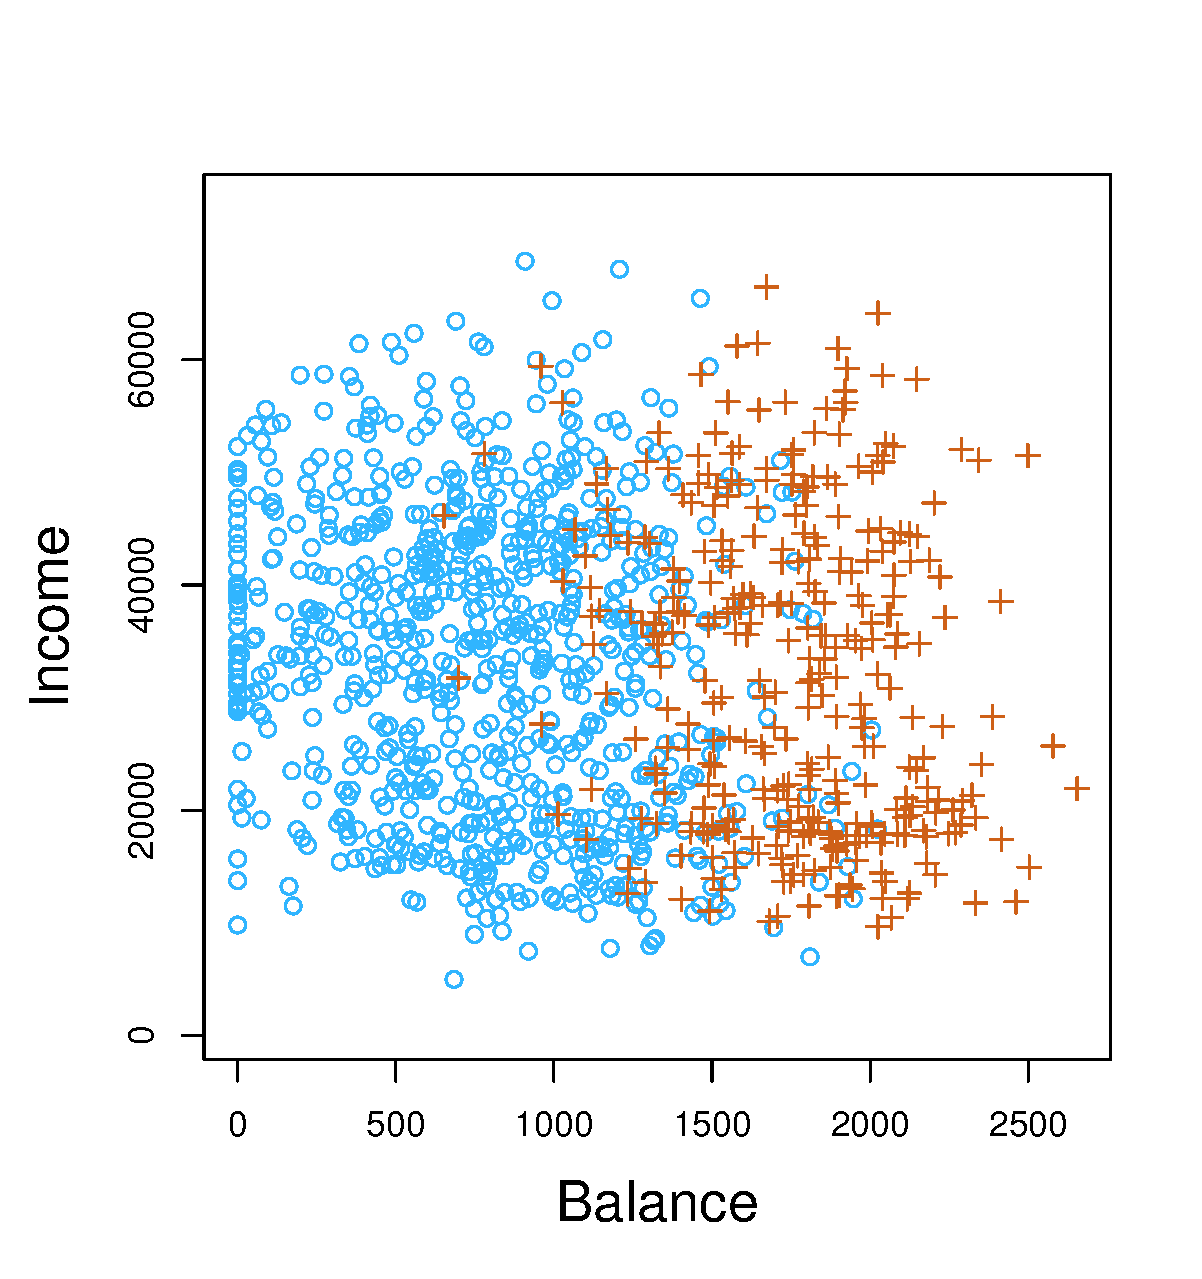
\includegraphics[width=0.34\textwidth]{4_1a}
		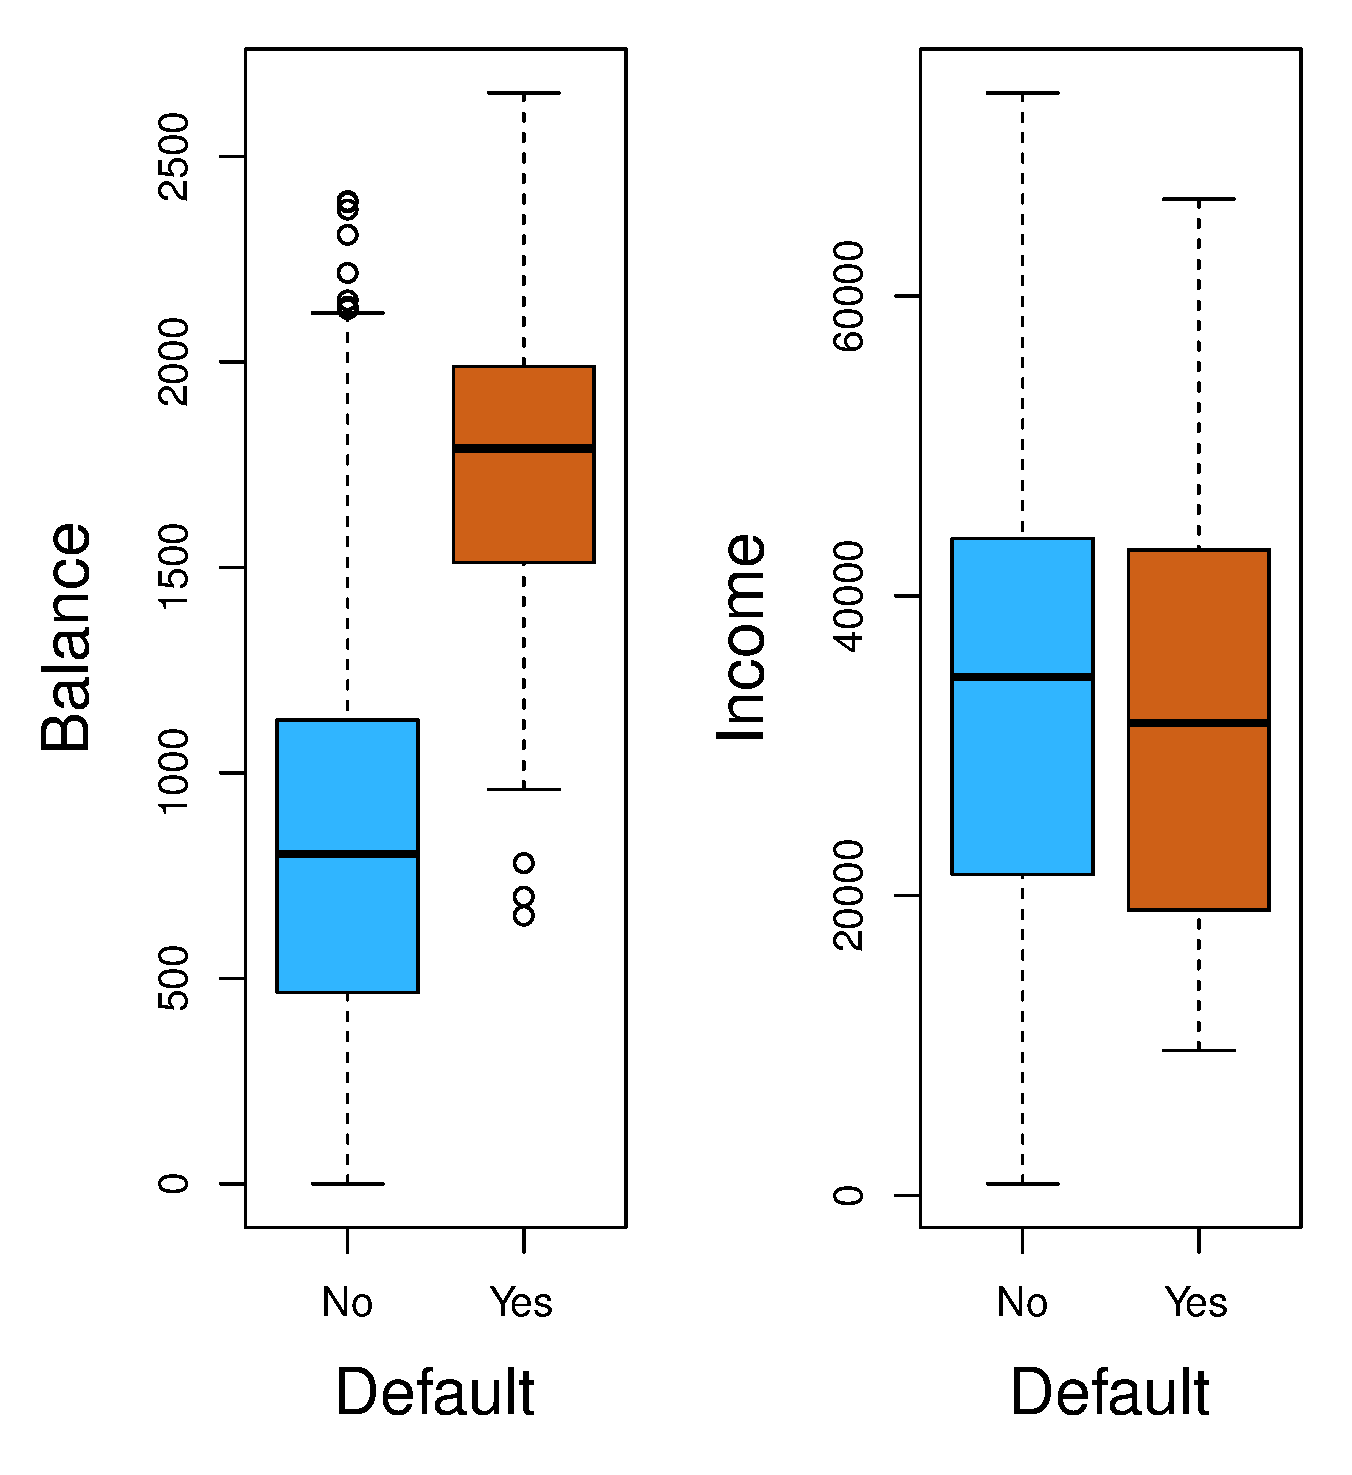
\includegraphics[width=0.3\textwidth]{4_1b}
	\end{center}

	Visualisation of the \dat{Default} data set. The classes are color coded.

	\bl{This is a simulated data set with an unusually high number of defaulters.}
\end{frame}

\begin{frame}{Example: Default Data Set}
	\begin{itemize}
		\item In this example the response is \e{binary}:
			\[
				y =
				\begin{cases}
					1 & \text{if \dat{default} is \val{Yes}} \\
					0 & \text{if \dat{default} is \val{No}} \\
				\end{cases}
			\]
		\item We encode qualitative responses the same way we encode qualitative predictors.
		\item Linear regression would work but is not ideal.
		\item \e{Logistic regression} is the superior method.
	\end{itemize}
	\bl{Logistic regression predicts probabilities.}
\end{frame}

\begin{frame}{Example: Default Data Set}
	\begin{itemize}
		\item For the \dat{Default} data set we would like to predict the probability
			of $\mdat{default} = \mval{Yes}$:
			\[ P(\mdat{default} = \mval{Yes} \vert \mdat{balance}) \]
		\item The probability is between $0$ and $1$.
		\item We can the \e{classify} based on $P$:
			\[ P(\mdat{default} = \mval{Yes} \vert \mdat{balance}) > 0.5\;:\; \mdat{default} = \mval{Yes} \]
	\end{itemize}
	\bl{we can of course choose different \e{working points}.}
\end{frame}

\begin{frame}{The Logistic Model}
	\begin{itemize}
		\item Out goal is to model the relationship
			\[ p(X) = P(Y=1\vert X) \leftrightarrow X \]
		\item We could use a linear regression model
			\[ p(X) = \beta_0 + \beta_1 X \]
		\item This does work but has some problems.
		\item In particular, the predicted probabilities can be $< 0$ or $> 1$.
	\end{itemize}
	\bl{We prefer a method that does not violate our axioms.}
\end{frame}

\begin{frame}{The Logistic Model}
	\begin{itemize}
		\item We must model $p(X)$ such that
			\[ p(X) \in \left[0, 1 \right] \;\;\forall X \]
		\item There a many functions that guarantee that.
		\item We use the \e{logistic function}
			\[ p(X) = \frac{e^{\beta_0 + \beta_1 X}}{ 1 + e^{\beta_0 + \beta_1 X}} \]
	\end{itemize}
	\bl{We will need a new fitting method for this.}
\end{frame}

\begin{frame}{The Logistic Model}
	\begin{center}
		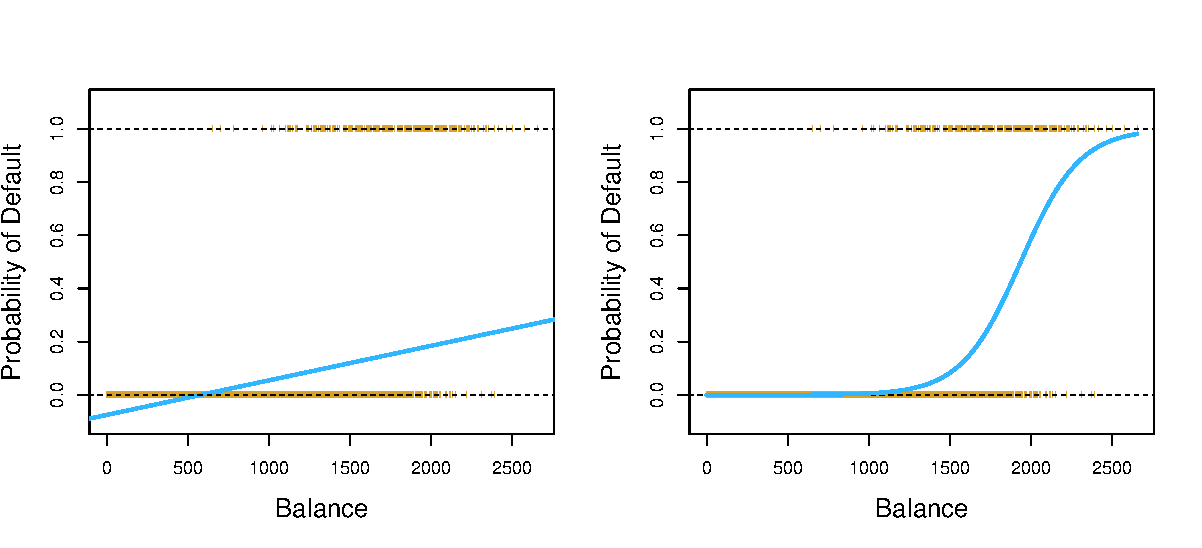
\includegraphics[width=0.8\textwidth]{4_2}

	Left: Linear Regression,
	Right: Logistic Regression
	\end{center}
	\bl{The logistic model satisfies our axioms.}
\end{frame}

\begin{frame}{The Logistic Model}
	\begin{itemize}
		\item The model looks complicated.
		\item How can we fit it?
		\item Some simple rearrangement yields the \e{odds}:
			\[ \frac{p(X)}{1 - p(X)} = e^{\beta_0 +\beta_1 X} \]
		\item For example:
			\[ p(0.2)\rightarrow\frac{1}{4}\;\;\;\;\text{and}\;\;\;\; p(0.9)\rightarrow 9 \]
	\end{itemize}
	\bl{Odds originate from betting on horse races.}
\end{frame}

\begin{frame}{The Logistic Model}
	\begin{itemize}
		\item How can the expression for the odds help us?
		\item How can we fit it?
		\item We take the logarithm of both sides to obtain
			\[ \log\left( \frac{p(X)}{1 - p(X)}\right)  = \beta_0 + \beta_1 X \]
		\item The left-hand side is called the \e{log odds} or \e{logit}.
	\end{itemize}
	\bl{The model for the logit is linear in $\bm{X}$.}
\end{frame}

\begin{frame}{The Logistic Model}
	\begin{itemize}
		\item  Recall that in linear regression $\beta_1$ describes the increase of $Y$ for
			a one-unit change in $X$.
		\item Here the interpretation is slightly more complicated.
		\item Changing $X$ by one unit changes the \e{logit} by $\beta_1$.
		\item Or equivalently, it multiplies the odds bt $e^{\beta_1}$.
		\item This does \e{not} imply a change of $\beta_1$ of $p(X)$!
		\item However, any \e{tendency} is preserved.
	\end{itemize}
	\bl{The logistic model has a nice interpretation.}
\end{frame}

\begin{frame}{The Logistic Model}
\end{frame}

\begin{frame}{Example: Default Data Set}
\end{frame}
\end{document}
